\section{Motivation}
\todo{Motivation}
Modern machine learning algorithms have reached a degree of potential that lets the resulting models model almost any dataset.
But even though there are statistical measures to guarantee that the model is learning correctly without over fitting on the training data, the model with the highest accuracy is not always the most usable model or even semantically correct.
The following three examples aim to showcase this:

\par \noindent (1)
\todo{pneumonia example}
% \cite{Caruana:2015:IMH:2783258.2788613}

\begin{figure}
\centering
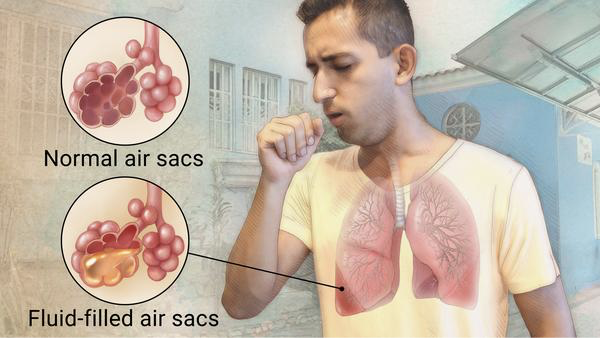
\includegraphics[height=6em,valign=t]{tex/introduction/pneumonia.png}
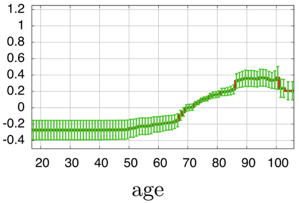
\includegraphics[height=8em,valign=t]{tex/introduction/age.png}
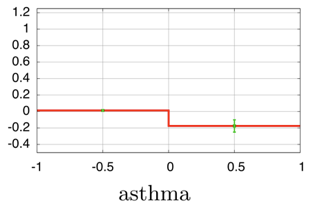
\includegraphics[height=8em,valign=t]{tex/introduction/asthma.png}
\caption{
\todo{TODO}
}
\label{figs:pneumonia}
\end{figure}

\par \noindent (2)
\todo{radio example}
% \cite{Bird:2002:ERI:1251972.1252349}
% https://people.duke.edu/~ng46/topics/evolved-radio.pdf

\begin{figure}
\centering
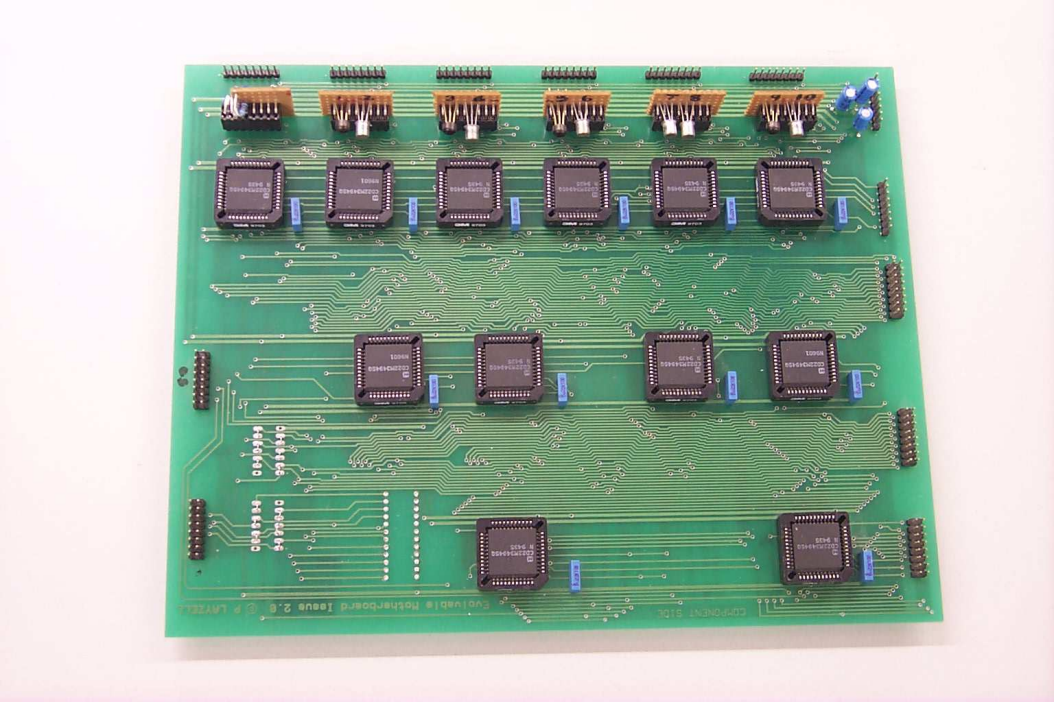
\includegraphics[height=10em]{tex/introduction/emradio.png}
\caption{
\todo{TODO}
}
\label{figs:emradio}
\end{figure}

\par \noindent (3)
\todo{toaster example}
% \cite{2017arXiv171209665B}
% https://arxiv.org/pdf/1712.09665.pdf

\begin{figure}
\centering
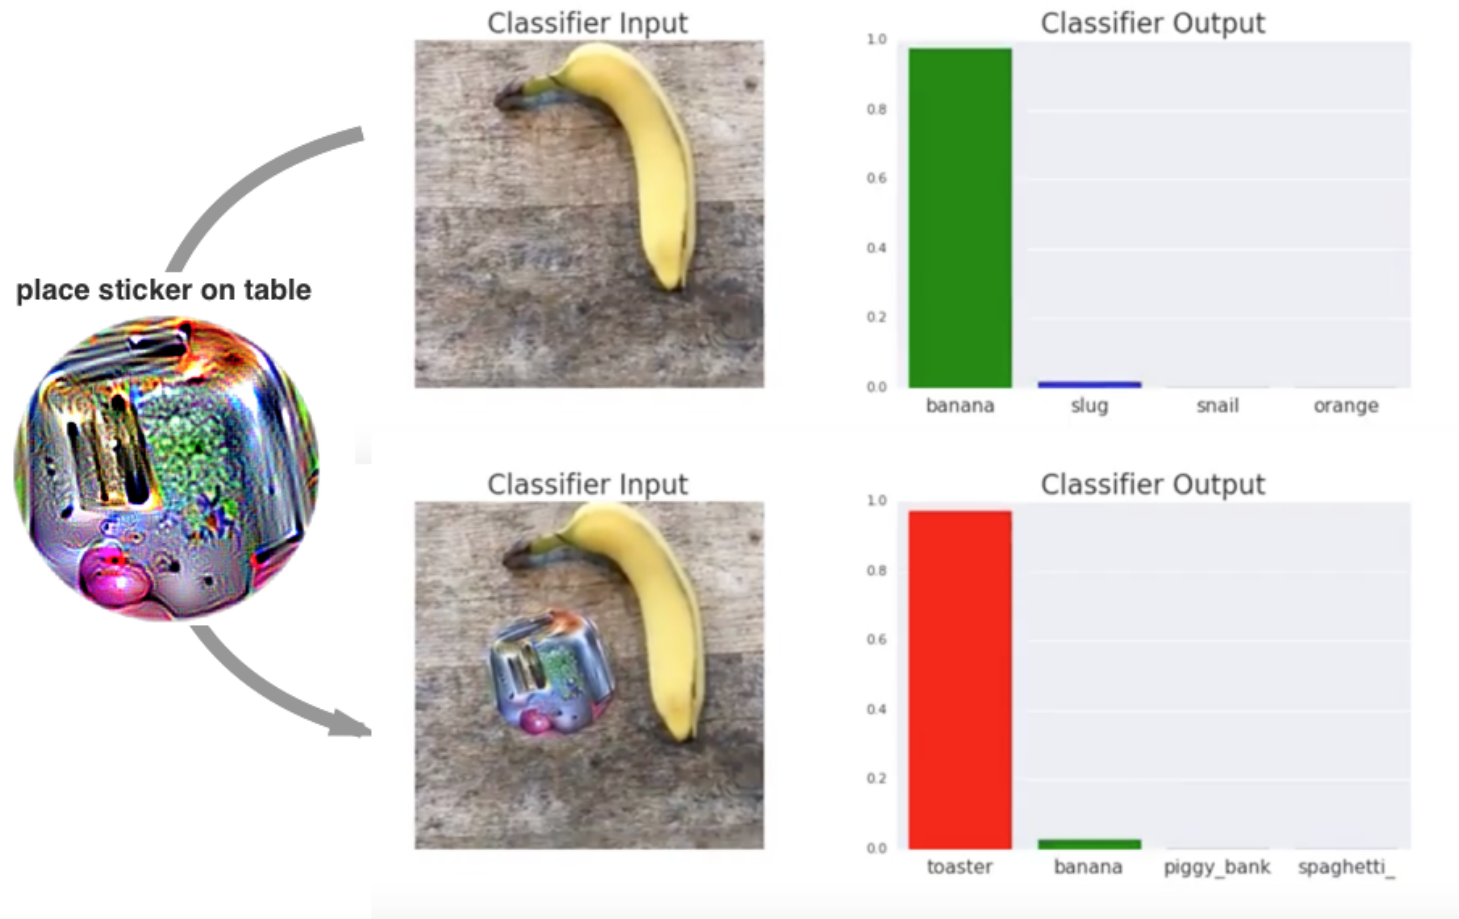
\includegraphics[height=10em]{tex/introduction/adversarialtoaster.png}
\caption{
\todo{TODO}
}
\label{figs:toaster}
\end{figure}

Those three examples all exhibit limitations of machine learning models where increasing the statistical accuracy of the model does not result in a semantically more correct model.
This is due to inherent biases of the data.

In the pneumonia example (1) patients with exceptionally high mortality risk were removed from the data leading to the model being unable to detect the severity of those cases.
In the radio example (2) the model utilized contextual data from the environment that is present but \emph{should} not be used in the model.
And in the toaster example (3) the model expected that all input data is coming from physical, real, objects.
Those biases cannot be detected from within the model or the data itself.
Furthermore, the process of detecting those errors, or even optimizing for semantic accuracy cannot be automated or be formulated as procedure, since there is no objective or measurable optimization criteria for it.
This is in contrast to statistical accuracy where a higher number always indicates a better model.
As a result, human judgment and contextual knowledge is absolutely necessary.

% There has been research...specialized models
In order for a technique to be effectively useful for a human it needs to have few restrictions \todo{}
* reasons for black box
\todo{problem statement}